% Options for packages loaded elsewhere
\PassOptionsToPackage{unicode}{hyperref}
\PassOptionsToPackage{hyphens}{url}
%
\documentclass[
  12pt,
  a4paper,
  DIV=11,
  numbers=noendperiod]{scrreprt}

\usepackage{amsmath,amssymb}
\usepackage{setspace}
\usepackage{iftex}
\ifPDFTeX
  \usepackage[T1]{fontenc}
  \usepackage[utf8]{inputenc}
  \usepackage{textcomp} % provide euro and other symbols
\else % if luatex or xetex
  \usepackage{unicode-math}
  \defaultfontfeatures{Scale=MatchLowercase}
  \defaultfontfeatures[\rmfamily]{Ligatures=TeX,Scale=1}
\fi
\usepackage{lmodern}
\ifPDFTeX\else  
    % xetex/luatex font selection
\fi
% Use upquote if available, for straight quotes in verbatim environments
\IfFileExists{upquote.sty}{\usepackage{upquote}}{}
\IfFileExists{microtype.sty}{% use microtype if available
  \usepackage[]{microtype}
  \UseMicrotypeSet[protrusion]{basicmath} % disable protrusion for tt fonts
}{}
\usepackage{xcolor}
\setlength{\emergencystretch}{3em} % prevent overfull lines
\setcounter{secnumdepth}{5}
% Make \paragraph and \subparagraph free-standing
\ifx\paragraph\undefined\else
  \let\oldparagraph\paragraph
  \renewcommand{\paragraph}[1]{\oldparagraph{#1}\mbox{}}
\fi
\ifx\subparagraph\undefined\else
  \let\oldsubparagraph\subparagraph
  \renewcommand{\subparagraph}[1]{\oldsubparagraph{#1}\mbox{}}
\fi


\providecommand{\tightlist}{%
  \setlength{\itemsep}{0pt}\setlength{\parskip}{0pt}}\usepackage{longtable,booktabs,array}
\usepackage{calc} % for calculating minipage widths
% Correct order of tables after \paragraph or \subparagraph
\usepackage{etoolbox}
\makeatletter
\patchcmd\longtable{\par}{\if@noskipsec\mbox{}\fi\par}{}{}
\makeatother
% Allow footnotes in longtable head/foot
\IfFileExists{footnotehyper.sty}{\usepackage{footnotehyper}}{\usepackage{footnote}}
\makesavenoteenv{longtable}
\usepackage{graphicx}
\makeatletter
\def\maxwidth{\ifdim\Gin@nat@width>\linewidth\linewidth\else\Gin@nat@width\fi}
\def\maxheight{\ifdim\Gin@nat@height>\textheight\textheight\else\Gin@nat@height\fi}
\makeatother
% Scale images if necessary, so that they will not overflow the page
% margins by default, and it is still possible to overwrite the defaults
% using explicit options in \includegraphics[width, height, ...]{}
\setkeys{Gin}{width=\maxwidth,height=\maxheight,keepaspectratio}
% Set default figure placement to htbp
\makeatletter
\def\fps@figure{htbp}
\makeatother

\KOMAoption{captions}{tableheading}
\usepackage{indentfirst}
\usepackage{float}
\floatplacement{figure}{H}
\usepackage[math,RM={Scale=0.94},SS={Scale=0.94},SScon={Scale=0.94},TT={Scale=MatchLowercase,FakeStretch=0.9},DefaultFeatures={Ligatures=Common}]{plex-otf}
\makeatletter
\@ifpackageloaded{caption}{}{\usepackage{caption}}
\AtBeginDocument{%
\ifdefined\contentsname
  \renewcommand*\contentsname{Содержание}
\else
  \newcommand\contentsname{Содержание}
\fi
\ifdefined\listfigurename
  \renewcommand*\listfigurename{Список иллюстраций}
\else
  \newcommand\listfigurename{Список иллюстраций}
\fi
\ifdefined\listtablename
  \renewcommand*\listtablename{Список таблиц}
\else
  \newcommand\listtablename{Список таблиц}
\fi
\ifdefined\figurename
  \renewcommand*\figurename{Рисунок}
\else
  \newcommand\figurename{Рисунок}
\fi
\ifdefined\tablename
  \renewcommand*\tablename{Таблица}
\else
  \newcommand\tablename{Таблица}
\fi
}
\@ifpackageloaded{float}{}{\usepackage{float}}
\floatstyle{ruled}
\@ifundefined{c@chapter}{\newfloat{codelisting}{h}{lop}}{\newfloat{codelisting}{h}{lop}[chapter]}
\floatname{codelisting}{Список}
\newcommand*\listoflistings{\listof{codelisting}{Листинги}}
\makeatother
\makeatletter
\makeatother
\makeatletter
\@ifpackageloaded{caption}{}{\usepackage{caption}}
\@ifpackageloaded{subcaption}{}{\usepackage{subcaption}}
\makeatother
\ifLuaTeX
\usepackage[bidi=basic]{babel}
\else
\usepackage[bidi=default]{babel}
\fi
\babelprovide[main,import]{russian}
\babelprovide[import]{english}
% get rid of language-specific shorthands (see #6817):
\let\LanguageShortHands\languageshorthands
\def\languageshorthands#1{}
\ifLuaTeX
  \usepackage{selnolig}  % disable illegal ligatures
\fi
\usepackage[style=gost-numeric,backend=biber,langhook=extras,autolang=other*]{biblatex}
\addbibresource{bib/cite.bib}
\usepackage{csquotes}
\usepackage{bookmark}

\IfFileExists{xurl.sty}{\usepackage{xurl}}{} % add URL line breaks if available
\urlstyle{same} % disable monospaced font for URLs
\hypersetup{
  pdftitle={Отчет по лабораторной работе 1},
  pdfauthor={Власов Артем Сергеевич},
  pdflang={ru-RU},
  hidelinks,
  pdfcreator={LaTeX via pandoc}}

\title{Отчет по лабораторной работе 1}
\usepackage{etoolbox}
\makeatletter
\providecommand{\subtitle}[1]{% add subtitle to \maketitle
  \apptocmd{\@title}{\par {\large #1 \par}}{}{}
}
\makeatother
\subtitle{Власов Артем Сергеевич}
\author{Власов Артем Сергеевич}
\date{}

\begin{document}
\maketitle

\renewcommand*\contentsname{Содержание}
{
\setcounter{tocdepth}{1}
\tableofcontents
}
\listoffigures
\listoftables
\setstretch{1.5}
\chapter{Цель
работы}\label{ux446ux435ux43bux44c-ux440ux430ux431ux43eux442ux44b}

Установить Rocky Linux на виртуальную машину.

\chapter{Задание}\label{ux437ux430ux434ux430ux43dux438ux435}

Установить и настроить опреационную систему, выполнить задание и
ответить на контрольные вопросы

\chapter{Выполнение лабораторной работы
1.}\label{ux432ux44bux43fux43eux43bux43dux435ux43dux438ux435-ux43bux430ux431ux43eux440ux430ux442ux43eux440ux43dux43eux439-ux440ux430ux431ux43eux442ux44b-1.}

Создадим новую виртуальную машину с помощью файла образа.

Создаем виртуальную машину. (\textbf{?@fig-001}).

\begin{figure}

{\centering 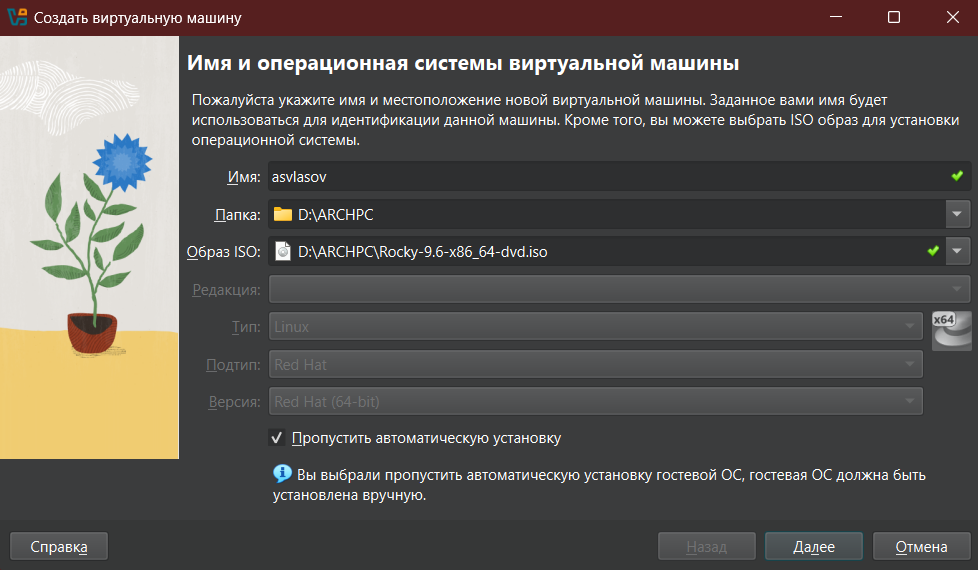
\includegraphics[width=0.7\textwidth,height=\textheight]{image/1.png}

}

\caption{Подключение образа}

\end{figure}%

Задаем первичные настройки машины. (\textbf{?@fig-002}).

\begin{figure}

{\centering 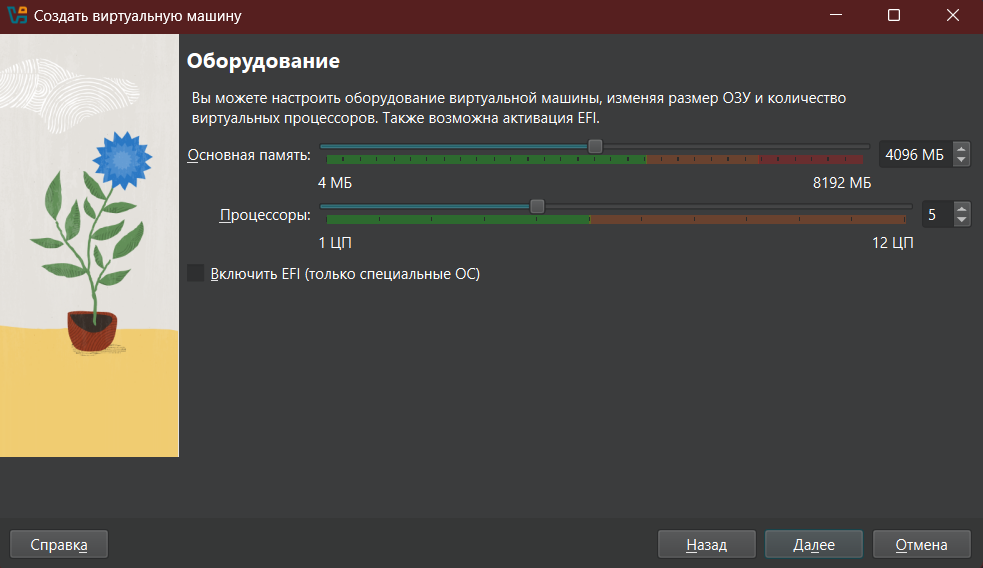
\includegraphics[width=0.7\textwidth,height=\textheight]{image/2.png}

}

\caption{Настраиваем ОЗУ и ядра процессора}

\end{figure}%%
\begin{figure}

{\centering 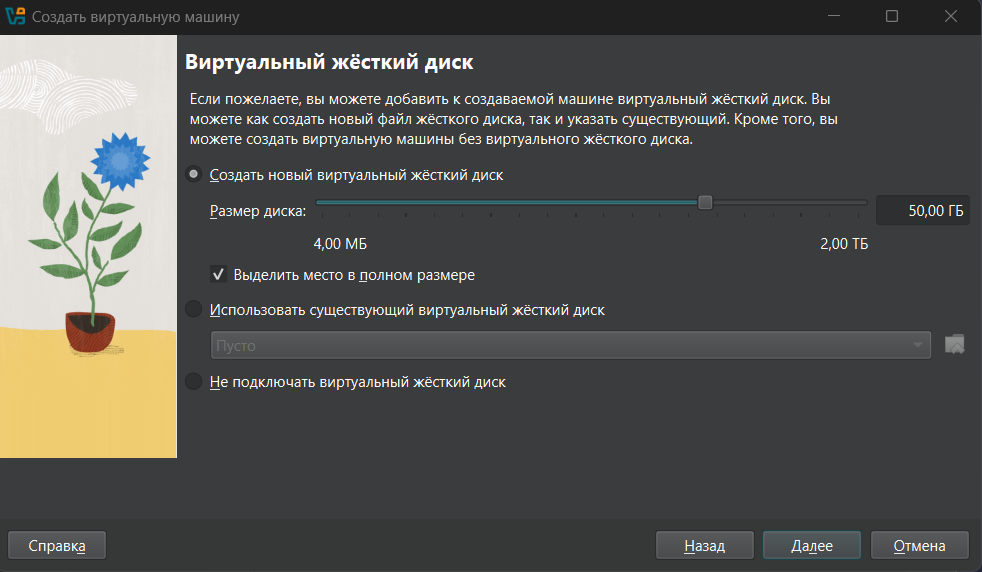
\includegraphics[width=0.7\textwidth,height=\textheight]{image/3.png}

}

\caption{Добавляем виртуальный диск}

\end{figure}%

Запуск и настройка ОС. (\textbf{?@fig-004}).

\begin{figure}

{\centering 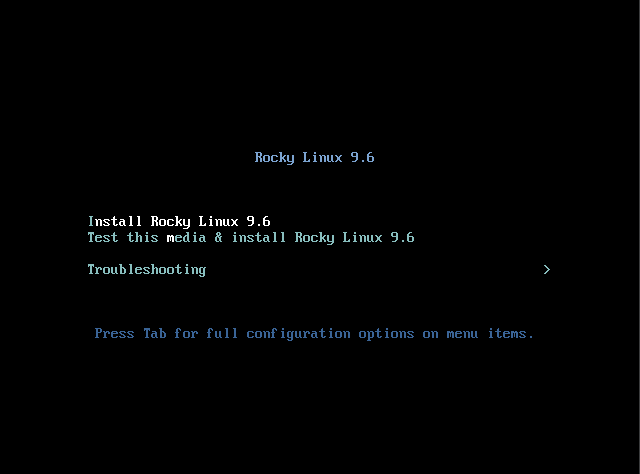
\includegraphics[width=0.7\textwidth,height=\textheight]{image/4.png}

}

\caption{Запуск}

\end{figure}%%
\begin{figure}

{\centering 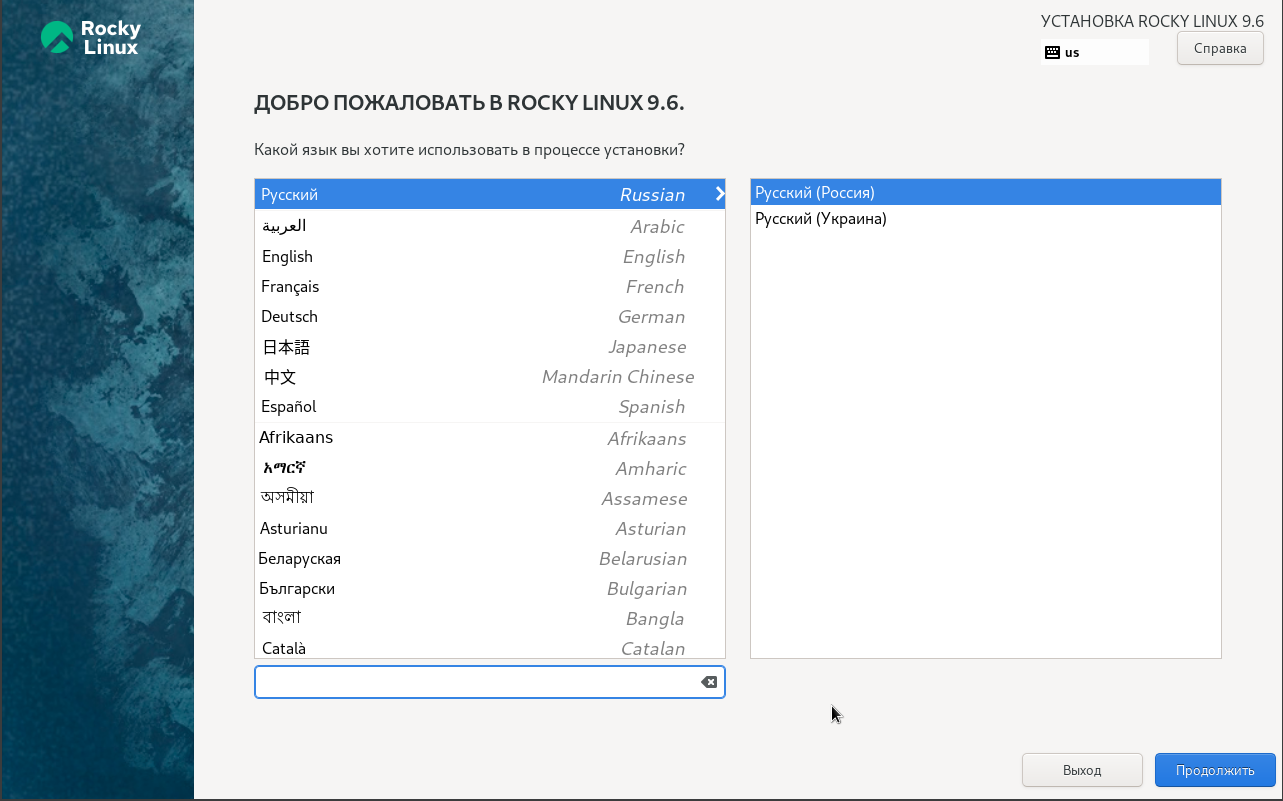
\includegraphics[width=0.7\textwidth,height=\textheight]{image/5.png}

}

\caption{Настрйока языка}

\end{figure}%%
\begin{figure}

{\centering 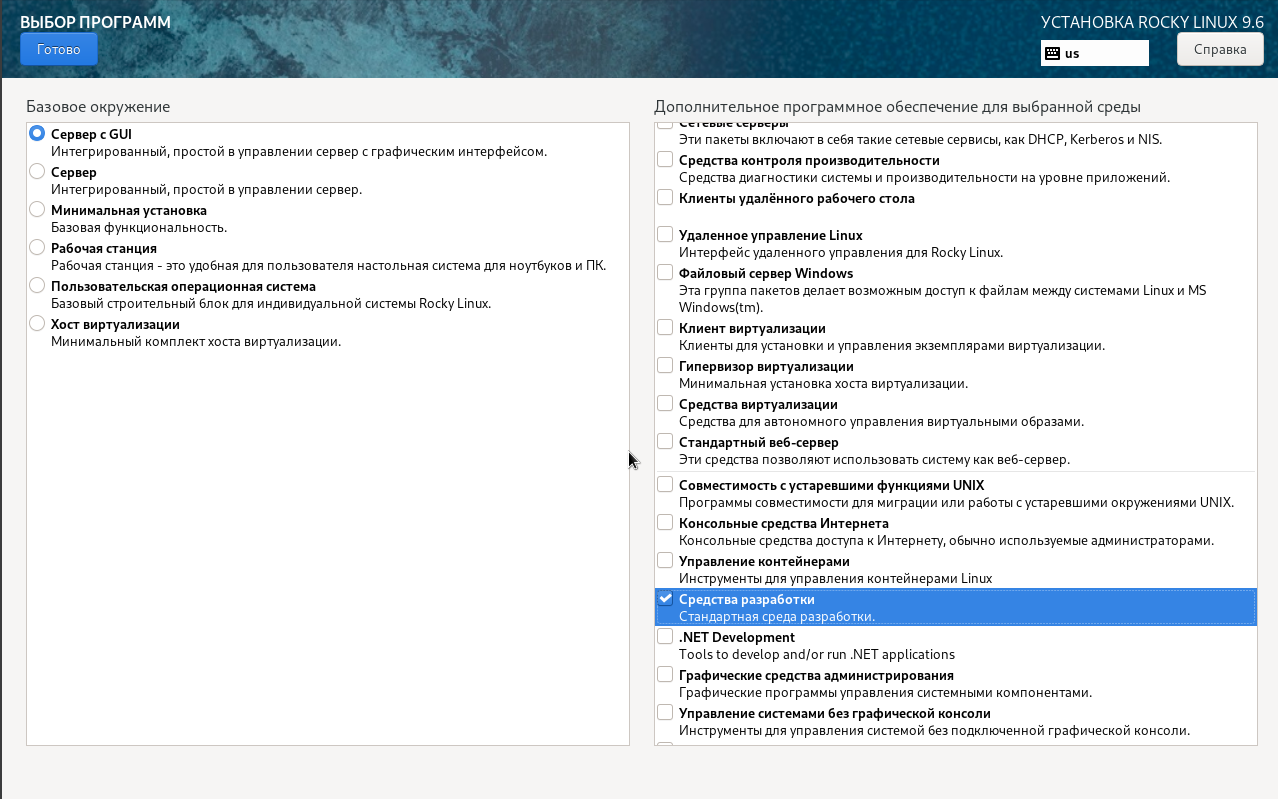
\includegraphics[width=0.7\textwidth,height=\textheight]{image/6.png}

}

\caption{Добавление стандартных утилит}

\end{figure}%%
\begin{figure}

{\centering 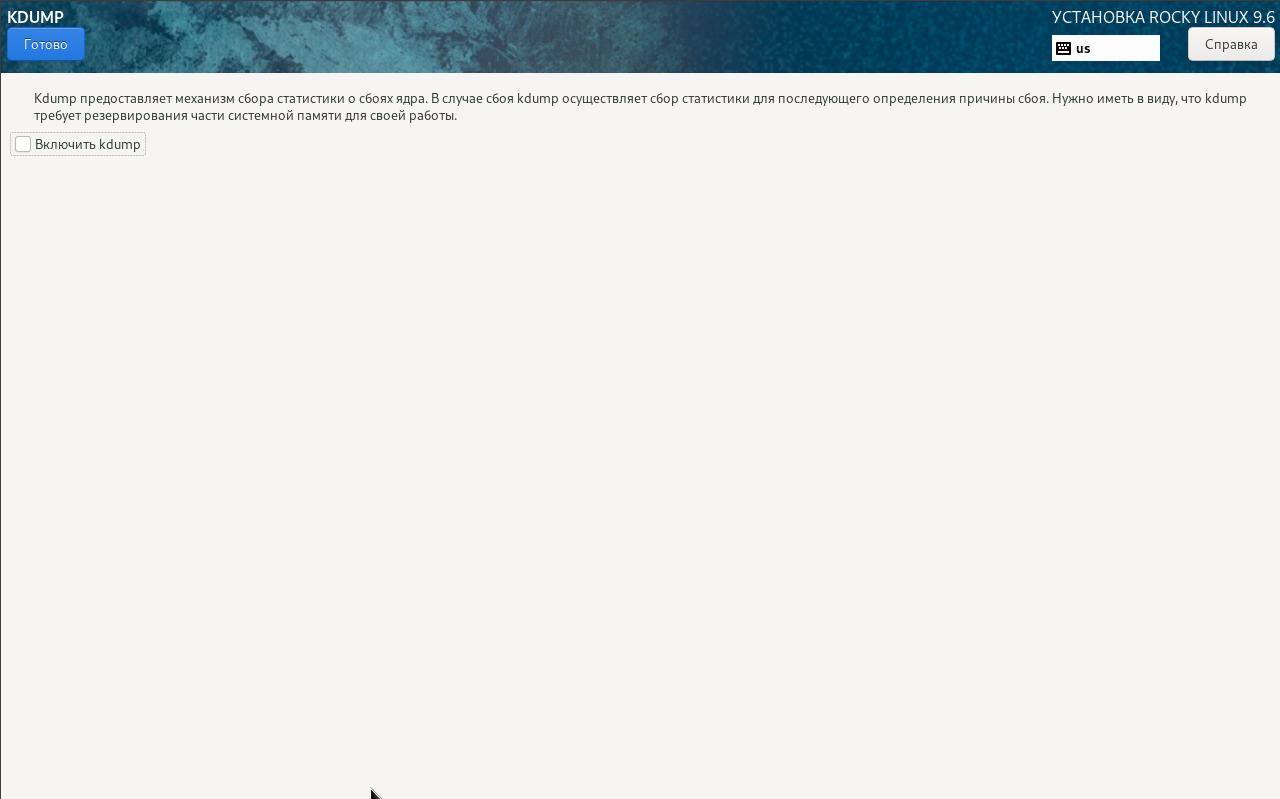
\includegraphics[width=0.7\textwidth,height=\textheight]{image/7.png}

}

\caption{Отключение KDUMP}

\end{figure}%%
\begin{figure}

{\centering 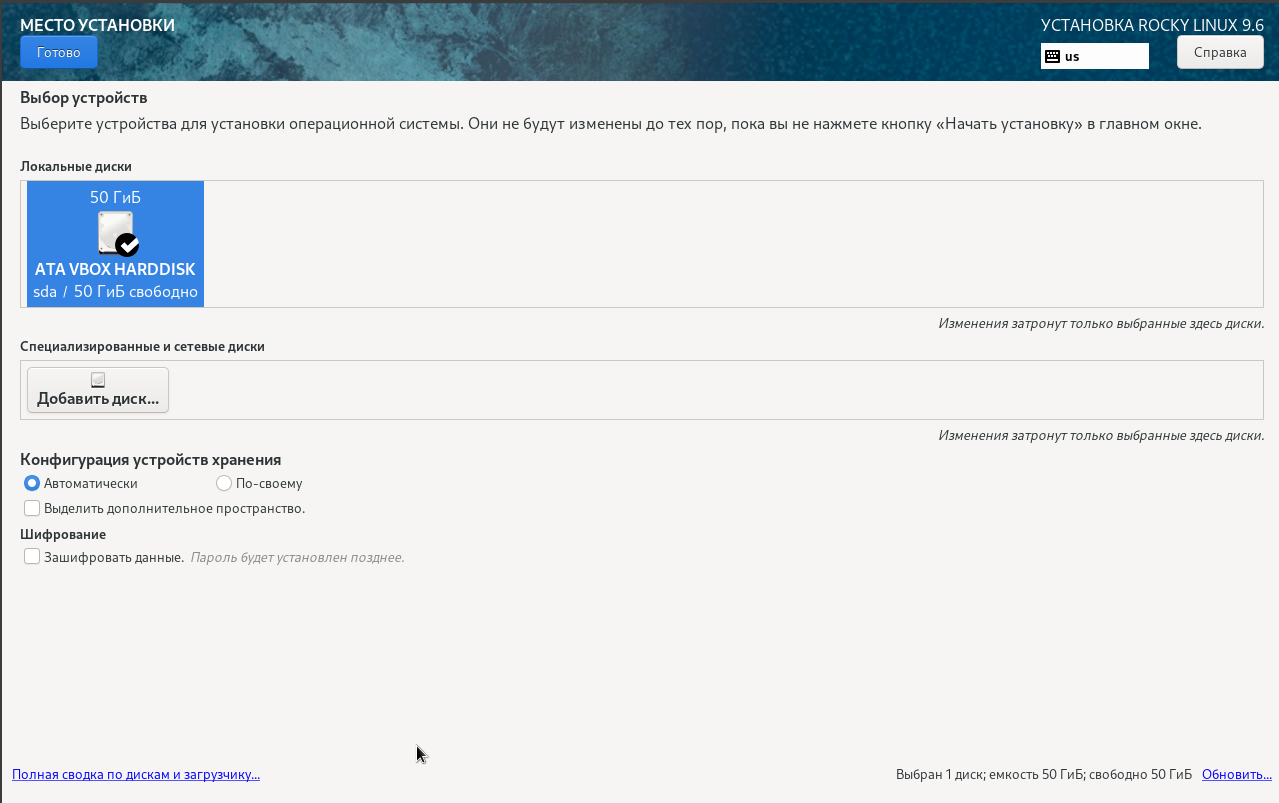
\includegraphics[width=0.7\textwidth,height=\textheight]{image/8.png}

}

\caption{Добавление диска}

\end{figure}%%
\begin{figure}

{\centering 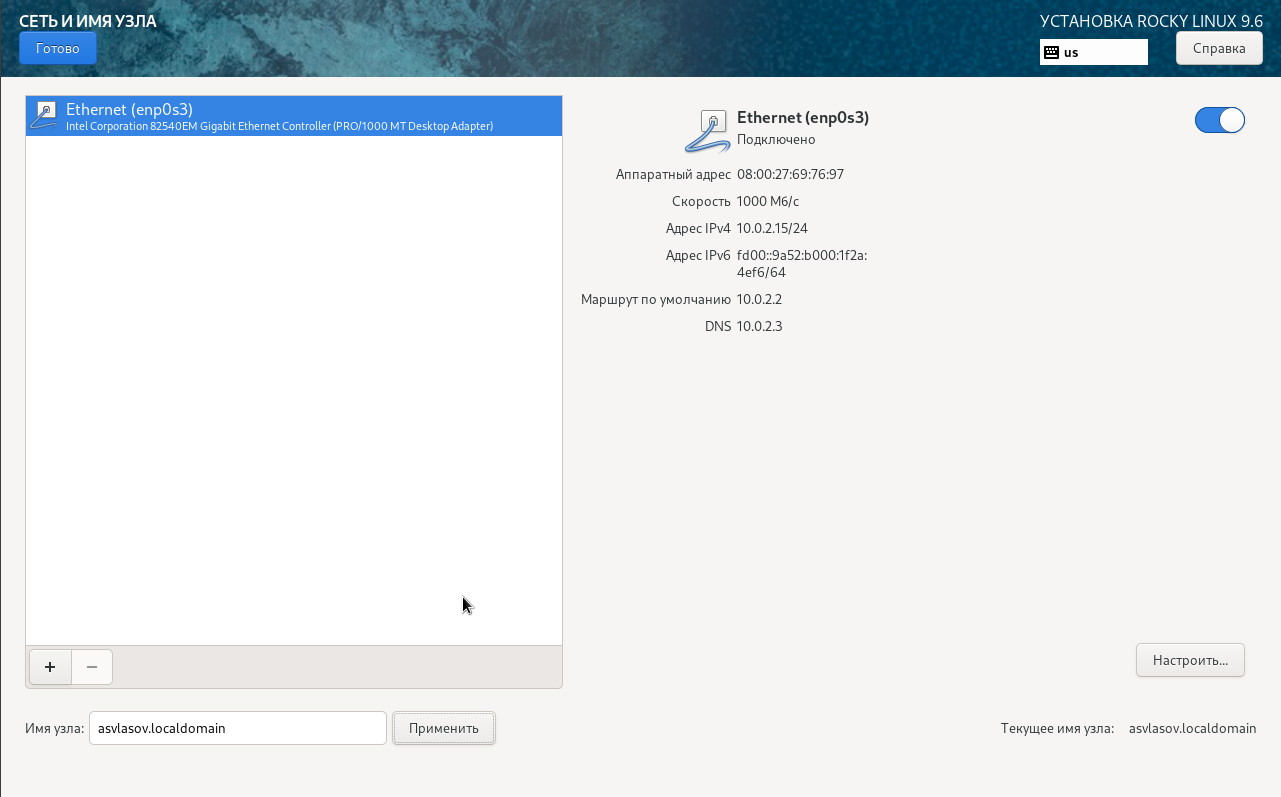
\includegraphics[width=0.7\textwidth,height=\textheight]{image/9.png}

}

\caption{Настройка сети}

\end{figure}%%
\begin{figure}

{\centering 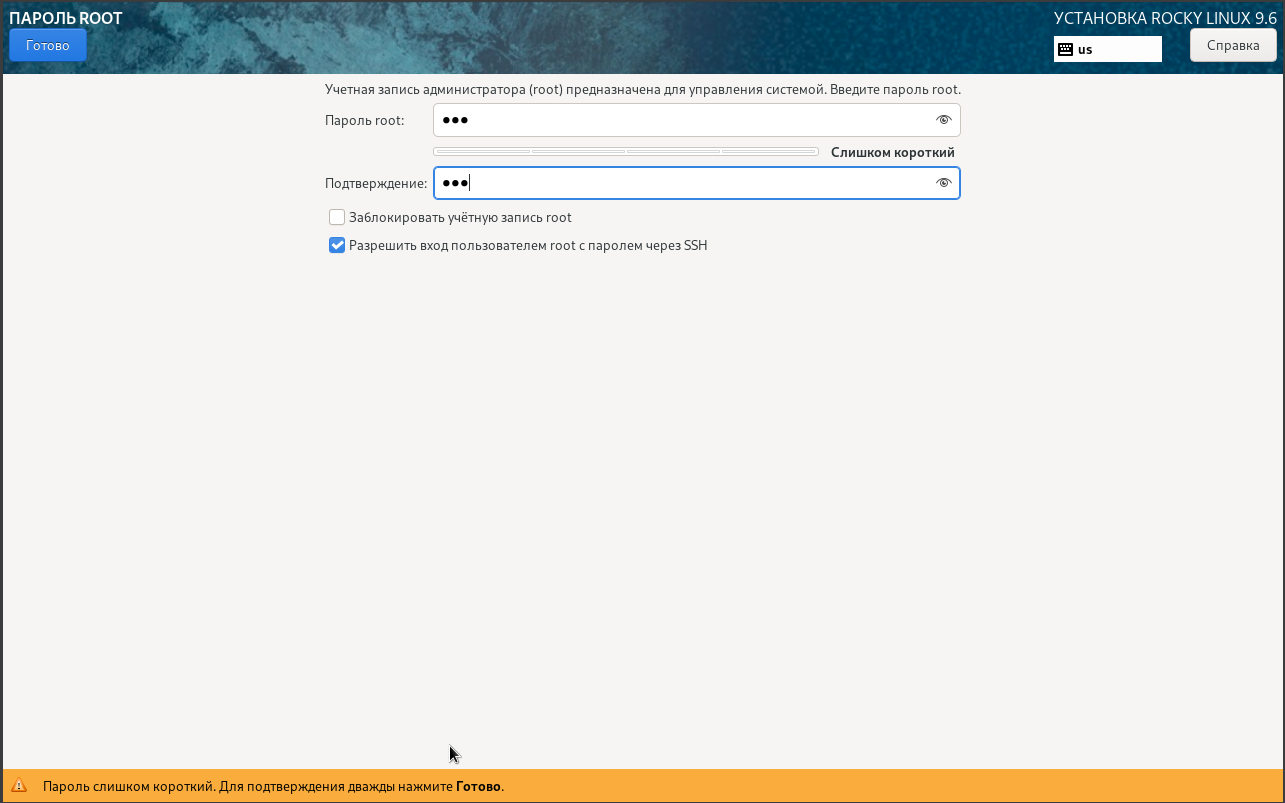
\includegraphics[width=0.7\textwidth,height=\textheight]{image/10.png}

}

\caption{ROOT}

\end{figure}%%
\begin{figure}

{\centering 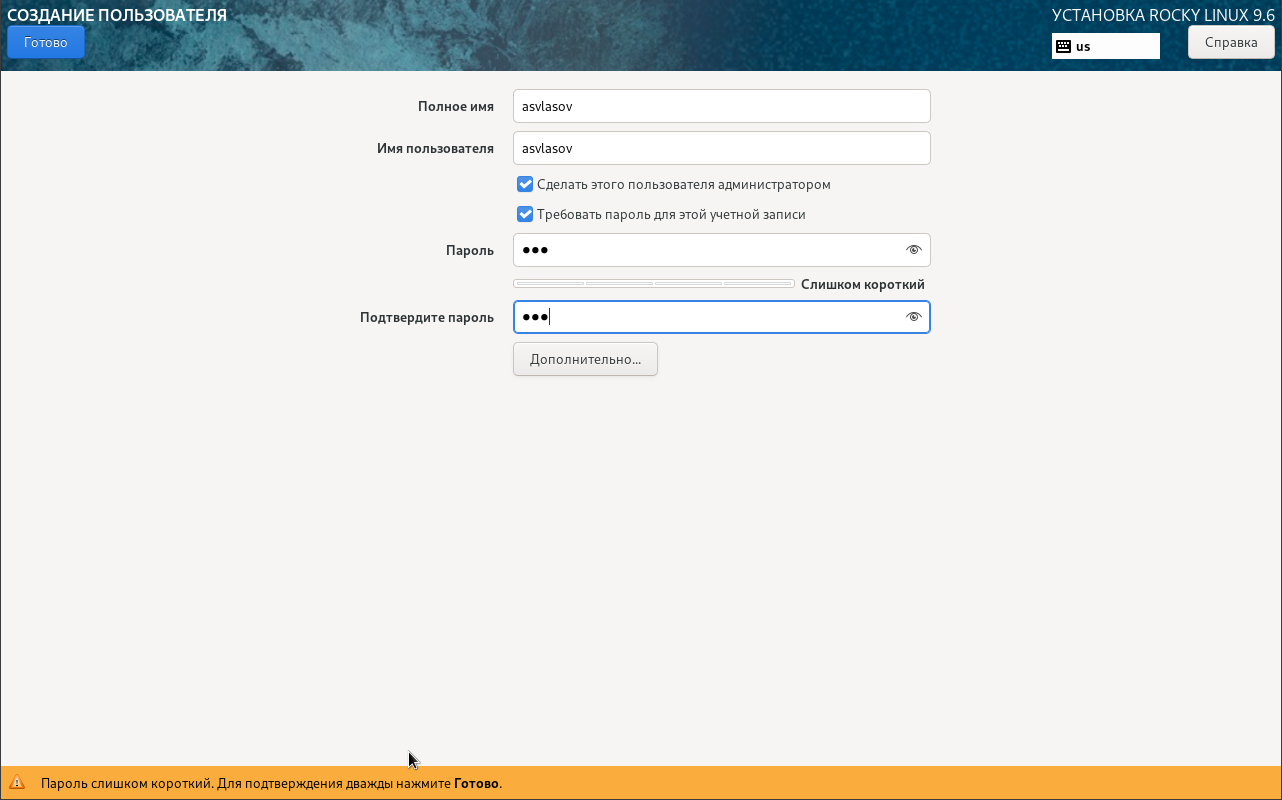
\includegraphics[width=0.7\textwidth,height=\textheight]{image/11.png}

}

\caption{Настройка пользователя}

\end{figure}%%
\begin{figure}

{\centering 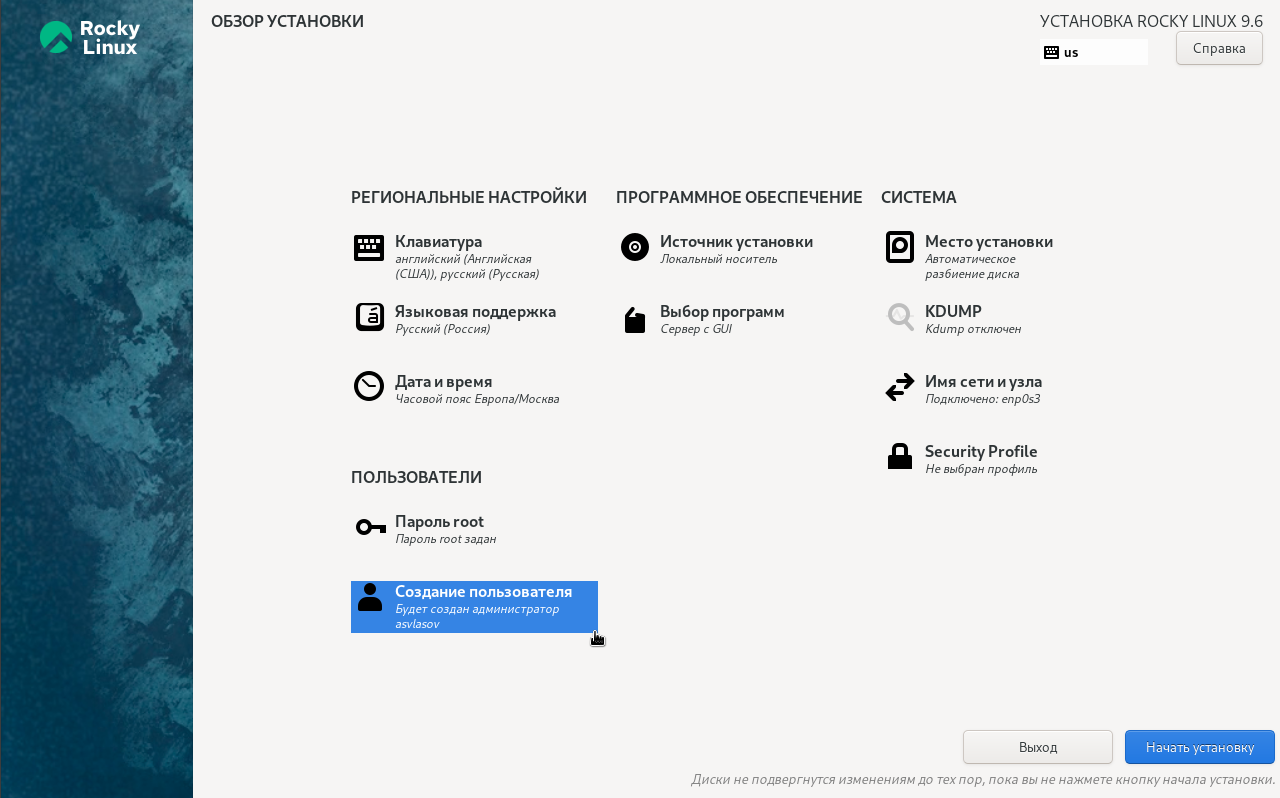
\includegraphics[width=0.7\textwidth,height=\textheight]{image/12.png}

}

\caption{Проверка всех настроек}

\end{figure}%%
\begin{figure}

{\centering 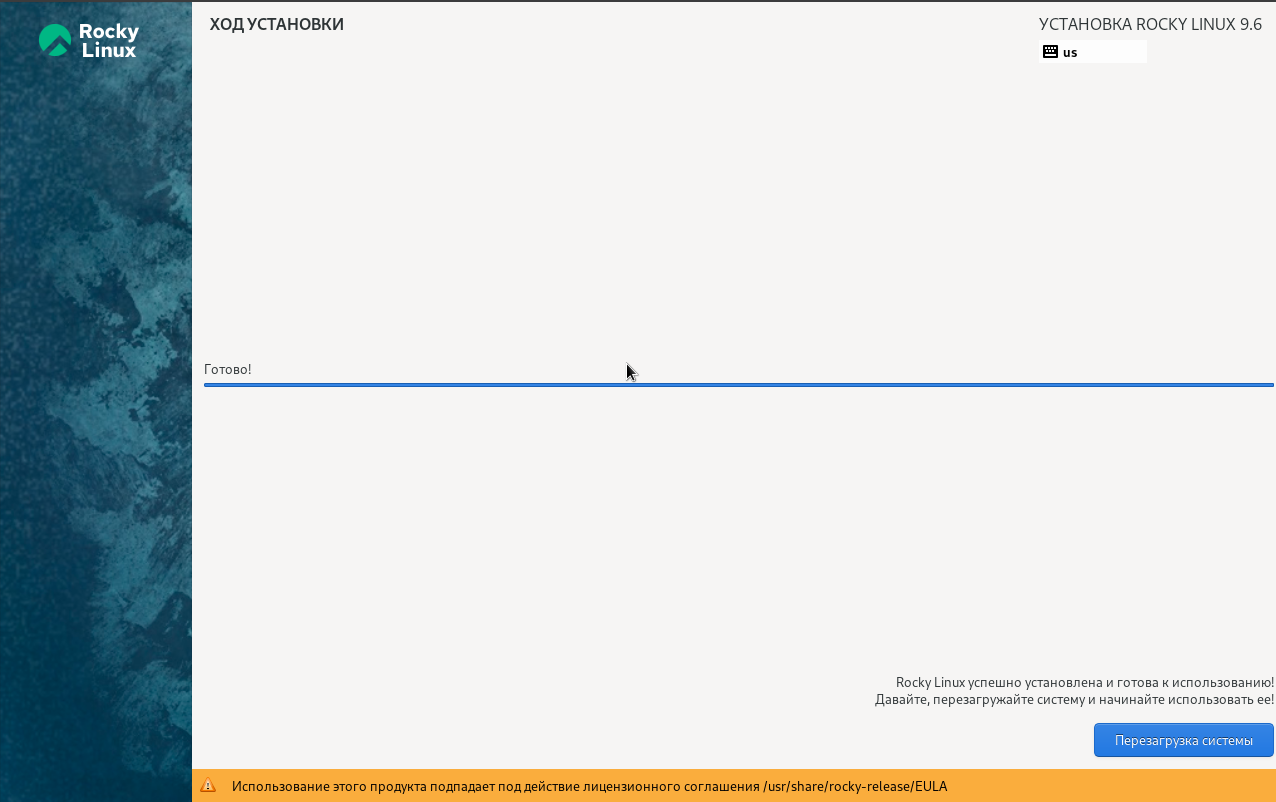
\includegraphics[width=0.7\textwidth,height=\textheight]{image/13.png}

}

\caption{Завершение установки}

\end{figure}%%
\begin{figure}

{\centering 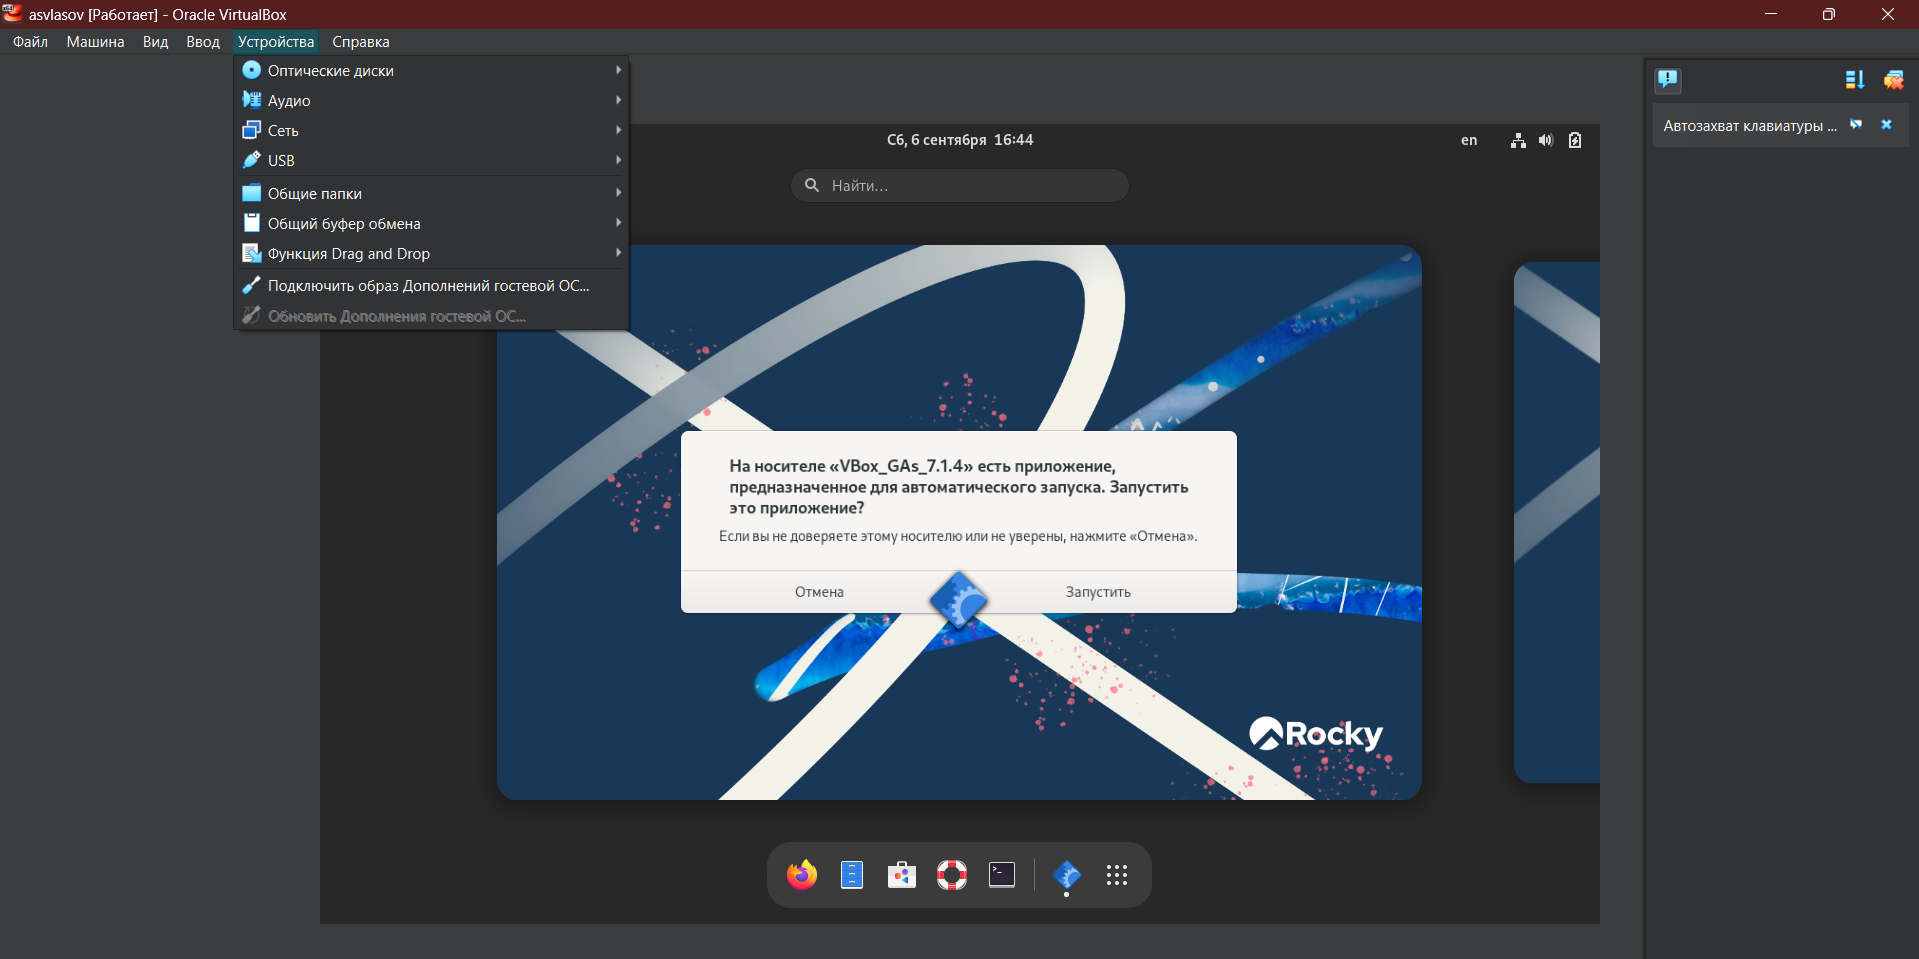
\includegraphics[width=0.7\textwidth,height=\textheight]{image/14.png}

}

\caption{Подключение образа дополнений гостевой ОС}

\end{figure}%

\#Выполение домашнего задания

\begin{figure}

{\centering 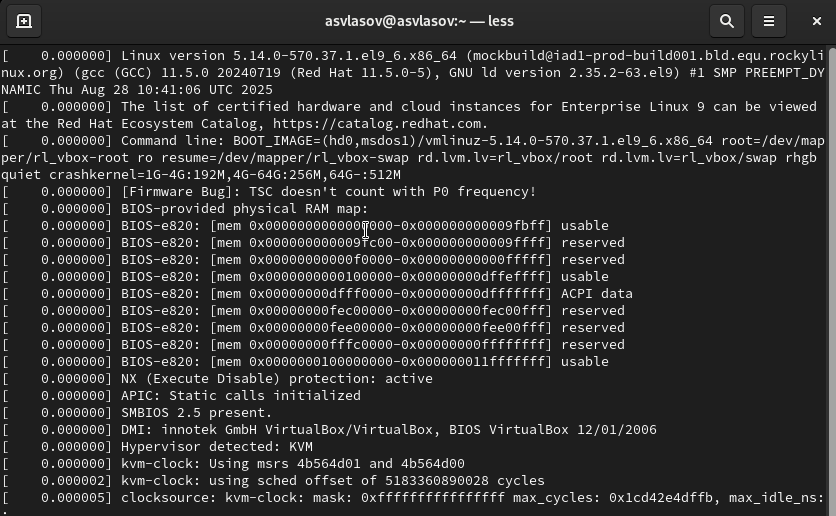
\includegraphics[width=0.7\textwidth,height=\textheight]{image/16.png}

}

\caption{Команда для просмотра технических характеристик}

\end{figure}%%
\begin{figure}

{\centering 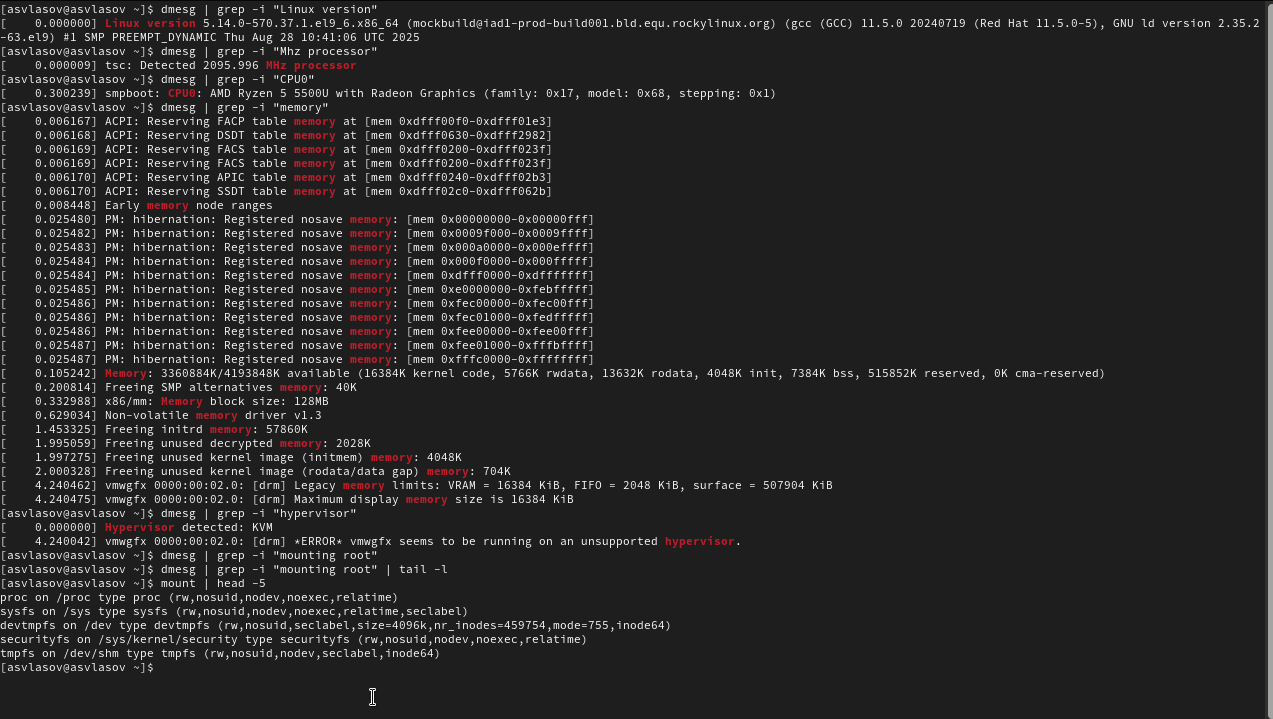
\includegraphics[width=0.7\textwidth,height=\textheight]{image/17.png}

}

\caption{Поиск семи элементов в тех. характеристиках}

\end{figure}%

\chapter{Контрольные
вопросы}\label{ux43aux43eux43dux442ux440ux43eux43bux44cux43dux44bux435-ux432ux43eux43fux440ux43eux441ux44b}

\section{1. Команды
терминала}\label{ux43aux43eux43cux430ux43dux434ux44b-ux442ux435ux440ux43cux438ux43dux430ux43bux430}

\subsection{• Для получения справки по
команде}\label{ux434ux43bux44f-ux43fux43eux43bux443ux447ux435ux43dux438ux44f-ux441ux43fux440ux430ux432ux43aux438-ux43fux43e-ux43aux43eux43cux430ux43dux434ux435}

\begin{itemize}
\tightlist
\item
  man - отображает официальное руководство\\
  Пример: man ls
  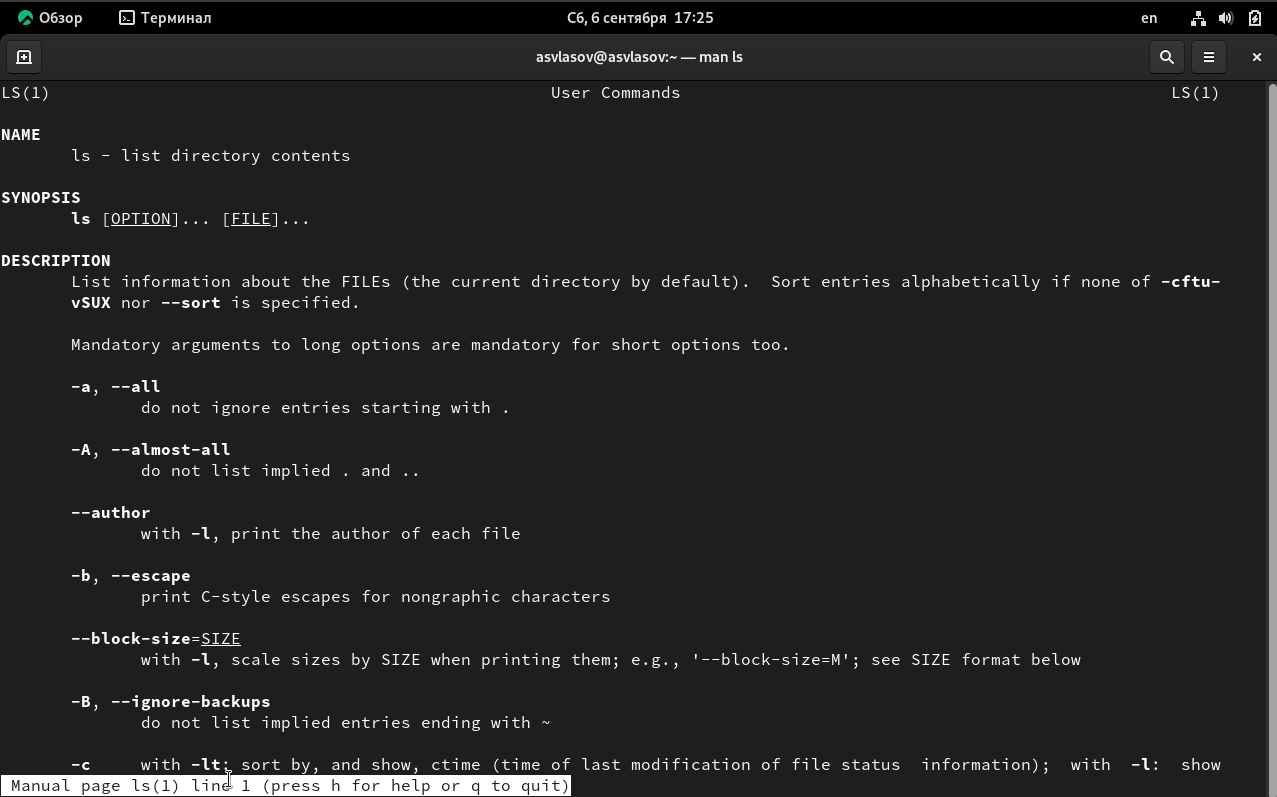
\includegraphics[width=0.7\textwidth,height=\textheight]{image/18.png}
\item
  --help или -h - краткая справка по использованию\\
  Пример: ls --help
\end{itemize}

\subsection{• Для перемещения по файловой
системе}\label{ux434ux43bux44f-ux43fux435ux440ux435ux43cux435ux449ux435ux43dux438ux44f-ux43fux43e-ux444ux430ux439ux43bux43eux432ux43eux439-ux441ux438ux441ux442ux435ux43cux435}

\begin{itemize}
\tightlist
\item
  pwd - показать текущую директорию\\
  Пример: pwd → /home/user
\item
  cd - сменить директорию\\
  Примеры: cd /var/log, cd \textasciitilde, cd .., cd -
  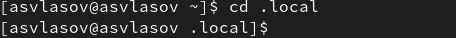
\includegraphics[width=0.7\textwidth,height=\textheight]{image/19.png}
\end{itemize}

\subsection{• Для просмотра содержимого
каталога}\label{ux434ux43bux44f-ux43fux440ux43eux441ux43cux43eux442ux440ux430-ux441ux43eux434ux435ux440ux436ux438ux43cux43eux433ux43e-ux43aux430ux442ux430ux43bux43eux433ux430}

\begin{itemize}
\tightlist
\item
  ls - список файлов и каталогов\\
  Примеры: ls, ls -l, ls -a, ls -lh, ls /etc
  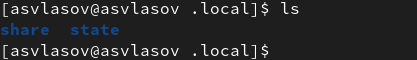
\includegraphics[width=0.7\textwidth,height=\textheight]{image/20.png}
\end{itemize}

\subsection{• Для определения объёма
каталога}\label{ux434ux43bux44f-ux43eux43fux440ux435ux434ux435ux43bux435ux43dux438ux44f-ux43eux431ux44aux451ux43cux430-ux43aux430ux442ux430ux43bux43eux433ux430}

\begin{itemize}
\tightlist
\item
  du - показывает занимаемый объём\\
  Примеры: du -sh /home/user, du -sh *, du -ah /dir
  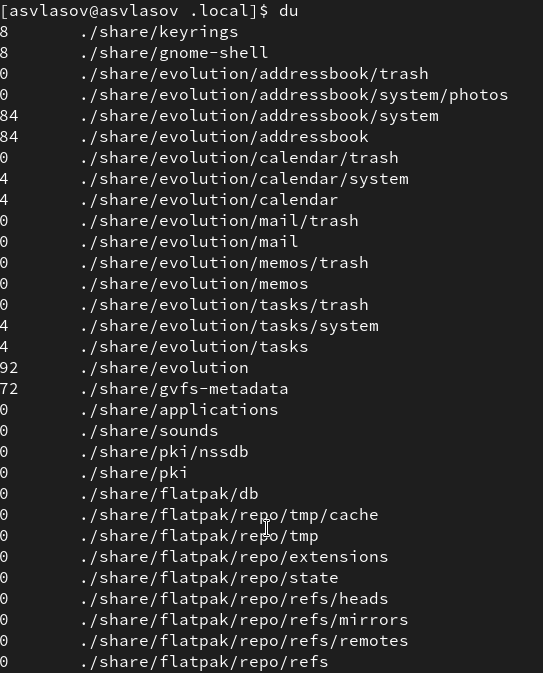
\includegraphics[width=0.7\textwidth,height=\textheight]{image/21.png}
\end{itemize}

\subsection{• Для создания/удаления
каталогов/файлов}\label{ux434ux43bux44f-ux441ux43eux437ux434ux430ux43dux438ux44fux443ux434ux430ux43bux435ux43dux438ux44f-ux43aux430ux442ux430ux43bux43eux433ux43eux432ux444ux430ux439ux43bux43eux432}

Создание: - mkdir - создать каталог\\
Пример: mkdir new\_folder - touch - создать файл\\
Пример: touch file.txt

Удаление: - rm - удалить файл\\
Пример: rm old\_file.txt - rm -r - удалить каталог рекурсивно\\
Пример: rm -r old\_folder
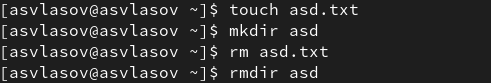
\includegraphics[width=0.7\textwidth,height=\textheight]{image/22.png}

\subsection{• Для задания определённых прав на
файл/каталог}\label{ux434ux43bux44f-ux437ux430ux434ux430ux43dux438ux44f-ux43eux43fux440ux435ux434ux435ux43bux451ux43dux43dux44bux445-ux43fux440ux430ux432-ux43dux430-ux444ux430ux439ux43bux43aux430ux442ux430ux43bux43eux433}

\begin{itemize}
\tightlist
\item
  chmod - изменяет права доступа\\
  Примеры (символьный метод):

  \begin{itemize}
  \tightlist
  \item
    chmod u+x script.sh - дать владельцу право на выполнение
  \item
    chmod go-w file.txt - забрать право на запись у группы и остальных
  \item
    chmod a+r file.txt - дать право на чтение всем
  \end{itemize}

  Пример (цифровой метод):

  \begin{itemize}
  \tightlist
  \item
    chmod 755 script.sh - владелец: rwx, группа: r-x, остальные: r-x
  \item
    chmod 644 config.txt - владелец: rw-, группа: r--, остальные: r--
    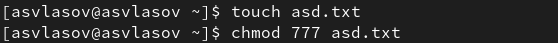
\includegraphics[width=0.7\textwidth,height=\textheight]{image/23.png}
  \end{itemize}
\end{itemize}

\subsection{• Для просмотра истории
команд}\label{ux434ux43bux44f-ux43fux440ux43eux441ux43cux43eux442ux440ux430-ux438ux441ux442ux43eux440ux438ux438-ux43aux43eux43cux430ux43dux434}

\begin{itemize}
\tightlist
\item
  history - выводит список всех выполненных команд с номерами
\item
  ! - выполнить команду из истории под указанным номером\\
  Пример: !205
\item
  !! - выполнить предыдущую команду
\item
  Ctrl + R - reverse search, поиск по истории команд
  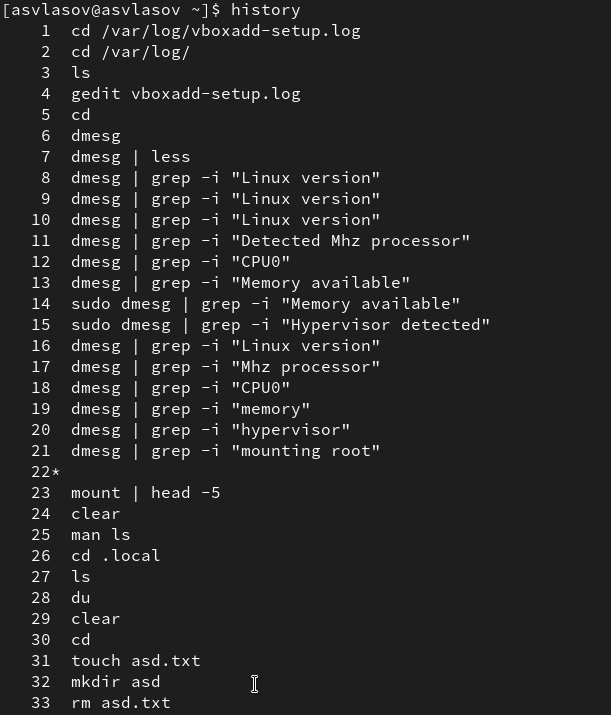
\includegraphics[width=0.7\textwidth,height=\textheight]{image/24.png}
\end{itemize}

\section{2. Учётная запись
пользователя}\label{ux443ux447ux451ux442ux43dux430ux44f-ux437ux430ux43fux438ux441ux44c-ux43fux43eux43bux44cux437ux43eux432ux430ux442ux435ux43bux44f}

Учётная запись пользователя содержит информацию: - Имя пользователя
(логин) - Зашифрованный пароль (хранится в /etc/shadow) - User ID (UID)
- уникальный числовой идентификатор - Group ID (GID) - идентификатор
основной группы - GECOS - комментарий (обычно ФИО) - Домашний каталог -
Командная оболочка (shell) по умолчанию

Команды для просмотра информации: - id - показывает UID, GID и группы
пользователя - whoami - показывает имя текущего пользователя - getent
passwd - отображает запись о пользователе
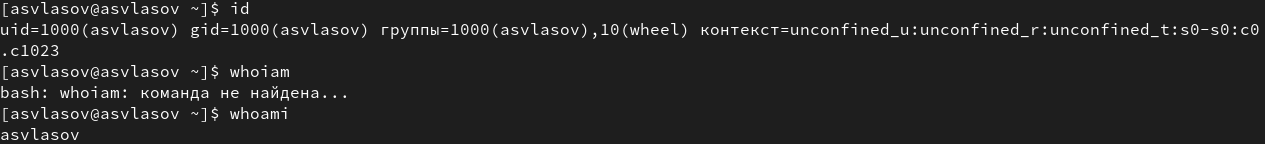
\includegraphics[width=0.7\textwidth,height=\textheight]{image/25.png}
\#\# 3. Файловая система

Файловая система - это способ организации, хранения и управления данными
на носителе.

Примеры с характеристикой: - ext4 - стандартная, надежная журналируемая
ФС для Linux - XFS - высокопроизводительная ФС, отлично для больших
файлов - Btrfs - современная ФС с поддержкой снимков и сжатия -
vfat/fat32 - простая ФС, совместимая с Windows, macOS и Linux

\section{4. Просмотр подмонтированных файловых
систем}\label{ux43fux440ux43eux441ux43cux43eux442ux440-ux43fux43eux434ux43cux43eux43dux442ux438ux440ux43eux432ux430ux43dux43dux44bux445-ux444ux430ux439ux43bux43eux432ux44bux445-ux441ux438ux441ux442ux435ux43c}

\begin{itemize}
\tightlist
\item
  mount - показывает все смонтированные файловые системы
\item
  findmnt - современная утилита, показывает дерево монтирования
\item
  df -h - показывает список ФС с размерами в удобном формате
  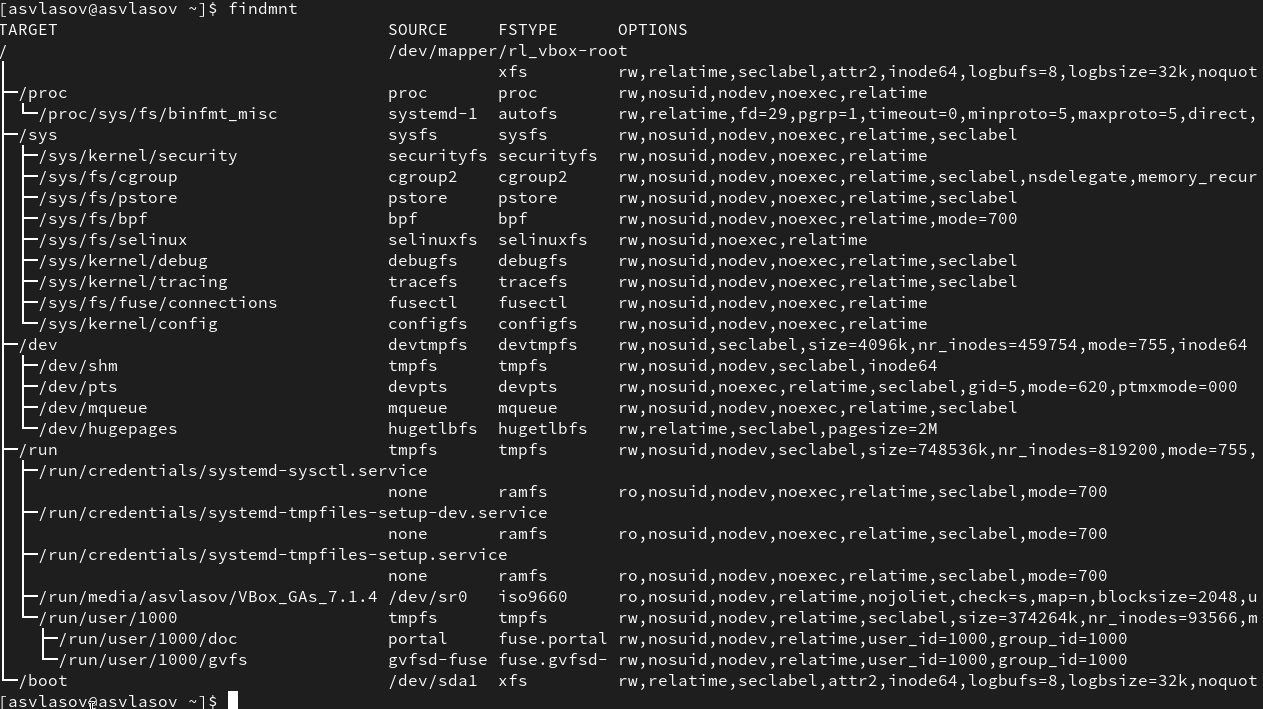
\includegraphics[width=0.7\textwidth,height=\textheight]{image/26.png}
  \#\# 5. Удаление зависшего процесса
\end{itemize}

\begin{enumerate}
\def\labelenumi{\arabic{enumi}.}
\tightlist
\item
  Найти PID процесса:

  \begin{itemize}
  \tightlist
  \item
    ps aux \textbar{} grep
  \item
    top или htop
  \end{itemize}
\item
  Завершить процесс:

  \begin{itemize}
  \tightlist
  \item
    kill - корректное завершение
  \item
    kill -9 - принудительное завершение
  \end{itemize}
\item
  Пример: ```bash ps aux \textbar{} grep firefox kill 1234 kill -9 1234
  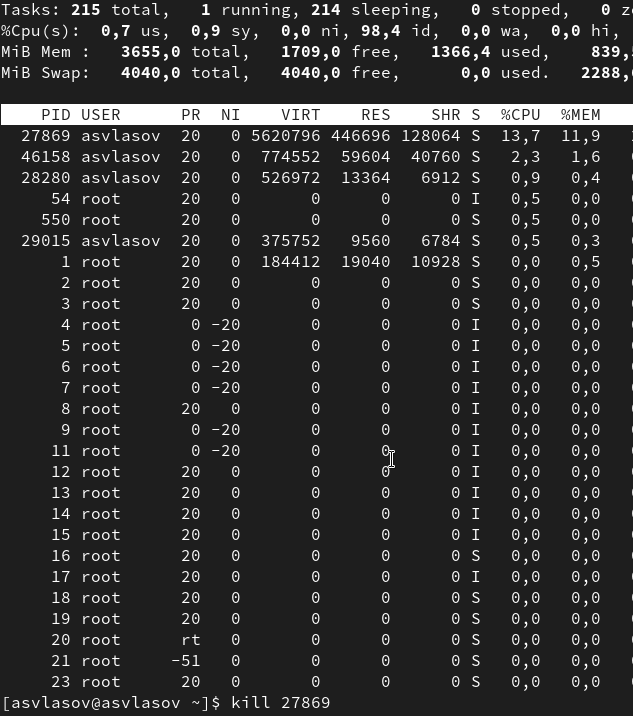
\includegraphics[width=0.7\textwidth,height=\textheight]{image/28.png}
\end{enumerate}

\chapter{Выводы}\label{ux432ux44bux432ux43eux434ux44b}

Мы установили ОС на виртуальную машину, выполнили задание и ответили на
контрольные вопросы.

\chapter*{Список
литературы}\label{ux441ux43fux438ux441ux43eux43a-ux43bux438ux442ux435ux440ux430ux442ux443ux440ux44b}
\addcontentsline{toc}{chapter}{Список литературы}

\printbibliography[heading=none]




\end{document}
